\documentclass[t]{beamer}
%% option to suppress auto-gen of document properties: usepdftitle=false
\usepackage[english]{babel}
%\usepackage{dcolumn}
\usepackage{bbold}
\usepackage{amsmath}
\usepackage{soul}
\usepackage{appendixnumberbeamer}

\usepackage{booktabs}
\usepackage{tabu}

\usepackage{tikz}
\usetikzlibrary{bayesnet}

\newcommand{\myemph}[1]{\alert{#1}}
\newcommand{\email}[1]{$\langle${#1}$\rangle$}
% \graphicspath{{../matlab/}}
% \newcolumntype{d}[1]{D{.}{.}{#1}}
\usepackage{hyperref}
\definecolor{myBlue}{rgb}{.75,.91,1}
\definecolor{myDarkBlue}{rgb}{0.0,0.0,0.55}
\definecolor{myRed}{rgb}{.698,.132,.132}
\definecolor{BrickRed}{rgb}{.698,.132,.132}
\definecolor{myGreen}{rgb}{.196,.804,.196}
\definecolor{BurntOrange}{rgb}{1,.648,0}
\definecolor{myGrey}{rgb}{.5,.5,.5}
\definecolor{LightCyan}{rgb}{0.88,1,1}

% Use "show notes" or "hide notes"
\setbeameroption{hide notes}

\mode<presentation>
{
  \usetheme{AnnArbor}
  \usecolortheme{default}
  \usefonttheme{default}
  \setbeamercovered{transparent}
  \setbeamerfont{downsize}{size=\footnotesize}
}
\mode<handout>
{
  \usetheme{default}
  \usecolortheme{default}
  \usefonttheme{default}
}
\AtBeginSection[]
{
  \begin{frame}
    \frametitle{Table of Contents}
    \tableofcontents[currentsection]
  \end{frame}
}
\title{Attentive Neural Processes}
\author[Derek Hansen]{Discussant: Derek Hansen}
\institute[UM Statistics]{\st{Probabilistic Machine Learning Reading Group} \\ \st{Applied Bayesian Reading Group} \\ {Computational Bayes Reading Group} \\ University of Michigan Department of Statistics}
\date{September 21, 2020}
\begin{document}

\frame{\titlepage}

\begin{frame}
  \frametitle{Motivating Example}
  \begin{itemize}
  \item https://youtu.be/fwWoBNELyeU?t=630
  \end{itemize}
  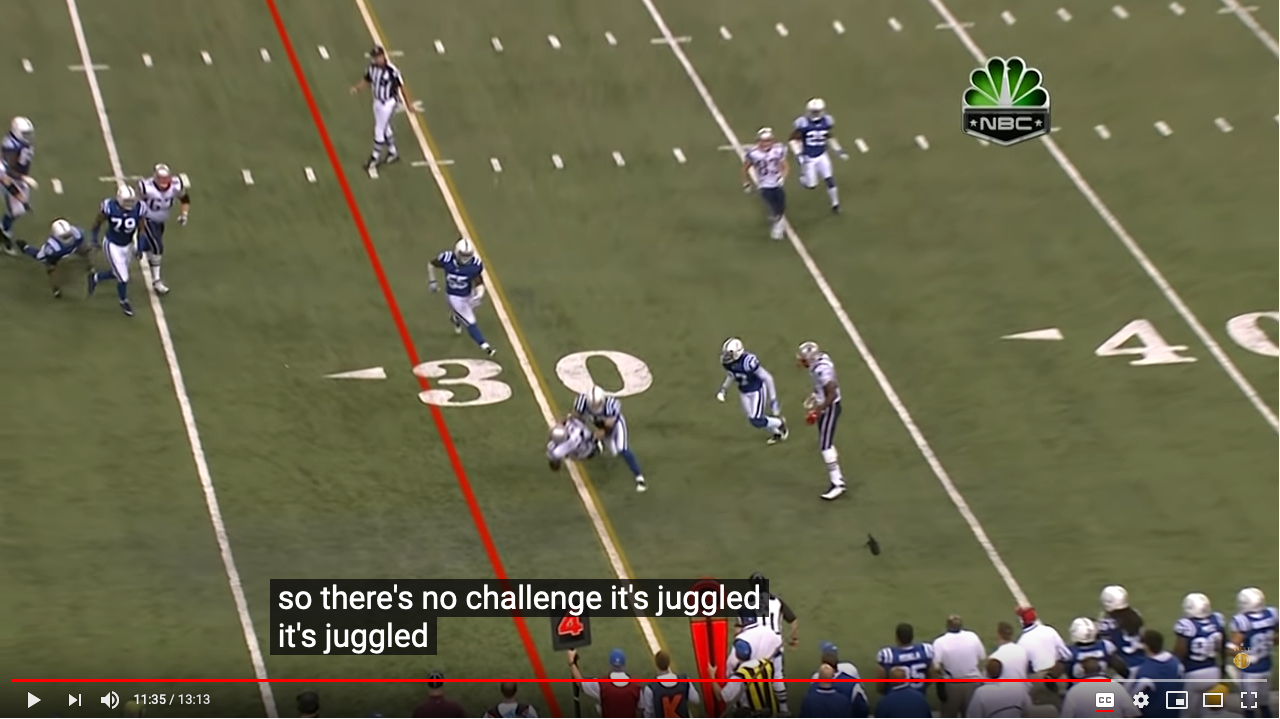
\includegraphics[width=\linewidth]{./motivating_example.png}
\end{frame}

\begin{frame}
  \frametitle{Overview}
  \tableofcontents
\end{frame}

\section{Neural Processes}

\begin{frame}
  \frametitle{Neural Process}
  \begin{itemize}
   \item We observe data $(x_i, y_i)$ where $x_i \in \mathbb R^{d_x}$ is a feature vector and $y_i \in \mathbb R^{d_y}$ is a label.
  \item The goal of the Neural Process is to learn a conditional distribution $p(y_i | x_i, r_C)$, where $i \in T$ is a member of the target set.
  \item The term $r_C \in \mathbb R^d$ parameterizes the conditional distribution. 
  \item $r_C$ is a finite-dimensional representation which is the output of a permutation-invariant function $r$:
    \[r_C \triangleq r\left( \{(x_j, y_i) | j \in C\} \right)\]
  \item $C$ is called the context set
  \item Generally $C \subset T$, so the goal is to use a subset of observations of a functional process to predict all points in the target set.
  \end{itemize}

\end{frame}

\begin{frame}
  \frametitle{Neural Process - generative model}
  \begin{itemize}
  \item The latent variable $z$ captures global uncertainty in the functional relationship between $x$ and $y$.
    \[
      \begin{split}
      p(y_i | x_i, \{(x_j, y_j) | j \in C\}) &= \int p_y(y_i | x_i, r_C, z) d p_z(z | \{(x_j, y_j) | j \in C\}) \\ 
      &= \int p_y(y_i | x_i, r_C, z) d p_z(z | s_C) \\
      s_C &= s( \{(x_j, y_j) | j \in C\}) 
    \end{split}
  \]
\item $s$ is another permutation-invariant function similar to $r$.
\item $p_z$ is referred to as the decoder \footnote{This is called $q$ in the ANP paper, but I'm not a fan of this notation.}, and $p_y$ is referred to as the encoder.
\item Allows for independent realizations of functions to be estimated together.
  \end{itemize}
\end{frame}


\begin{frame}
  \frametitle{Neural Process - inference}
  \begin{itemize}
  \item For inference, we pick a variational distribution for the latent $z$ which can depend on the entire target set.
    \[
      \begin{split}
      q(z | \{(x_i, y_i) | i \in  T\}) &= q(z | s_T) \\
                                        &\triangleq p_z(z | s_T)
                                      \end{split}
      \] where $s_T \triangleq s(\{(x_i, y_i) | i \in T\})$
  \item We then maximize the ELBO:
    \[
      \begin{split}
        &\mathbb E_{q(z | s_T)} (\sum_{i \in T} \log p_y(y_i | x_i, r_C, z) p_z(z | s_C)) - \mathbb E_{q(z | s_T)} \log q(z | s_T)\\
        &= \sum_{i \in T} \mathbb E_{q(z | s_T)} \log p_y(y_i | x_i, r_C, z) + \mathbb E_{q(z|s_T)} \log p_z(z|s_C) \\
        &-  \mathbb E_{q(z | s_T)} \log q(z | s_T)\\
        &= \sum_{i \in T} \mathbb E_{q(z | s_T)} \log p_y(y_i | x_i, r_C, z) - D_{\mathrm{KL}} (q(z|s_T) \| p_z(z | s_C)) 
   \end{split}
    \]
                                    
  \end{itemize}
 \end{frame}

 \begin{frame}
   \frametitle{Neural Process - visualization}
   % \begin{figure}
   %   \centering
   \includegraphics[width=\linewidth]{./anp/np_dag.png}
   % \caption{Taken from Garnelo et al. 2018}
   % \end{figure}
   \centering From Garnelo et al. 2018.
   \begin{itemize}
   \item Note: In the original Neural Process, the predictions only depend on the
     context set through the latent $z$. ($r_C$ and $r_T$ above would read $s_C$ and $s_T$ in our current formulation)
   \end{itemize}
 \end{frame}

 
 \begin{frame}
   \frametitle{Neural Process - training}
   \begin{itemize}
   \item During training, the selection of the context set $C$ is randomized as well.
   \item Hence, the Neural Process does not present a fully generative model for all observed labels $Y_i$.
     Instead, it is a conditional model.
   \item This means that the learned data-generating process is not consistent. The learned conditional models do not follow the rules.
    \item Example: Suppose we have three observed data-points $(x_i, y_i), i = 1,2,3$.
     \[
       \begin{split}
         &p_\theta((y_3, y_2) | x_3, x_2, \{(x_1, y_1)\}) \ne \\
         &p_\theta(y_3 | x_3, \{(x_1, y_1), (x_2, y_2)\}) p_\theta(y_2 | x_2, \{(x_1, y_1)\})
     \end{split}
   \]
   \item This breaks Bayes' rule that $P(y_3, y_2 | y_1) = P(y_3 | y_2, y_1) P(y_2 | y_1)$.
   \end{itemize}
 \end{frame}

\section{Attention and self-attention}

\begin{frame}
  \frametitle{Attention (Scaled Dot-Product)}
  \begin{itemize}
  % \item In computer science, a dictionary is a structure which maps \textbf{keys} to \textbf{values}.
  \item An attention mechanism has three main ingredients:
    \begin{itemize}
    \item Query: $Q=[q_1 | \dots | q_{d_q}]^\top$
    \item Key : $K=[k_1 | \dots | q_{d_k}]^\top$
      \item Value $V=[v_1 | \dots | v_{d_k}]^\top$
    \end{itemize}
  \item $\mathrm{Attention}(Q, K, V) = \mathrm{softmax} \left( \frac{QK^\top}{\sqrt{d_k}} \right)V$.
  \item $\mathrm{softmax} \left( \begin{bmatrix} x_{1,1} & \dots & x_{1, n} \\ \vdots & \ddots & \vdots \\ x_{m, 1} & \dots & x_{m,n} \end{bmatrix} \right) = \begin{bmatrix} \frac{\exp(x_{1,1})}{\sum_{i=j}^n \exp(x_{1, j})} & \dots & \frac{\exp(x_{1, n})}{\sum_{j=1}^n\exp(x_{1, j})} \\ \vdots & \ddots & \vdots \\ \frac{\exp(x_{m, 1})}{\sum_{i=1}^m \exp(x_{m, j})} & \dots & \frac{\exp(x_{m,n})}{\sum_{j=1}^n \exp(x_{m, j})} \end{bmatrix}$
  \item Let $X \triangleq \mathrm{softmax} (QK^\top / \sqrt {d_k})$. Let $Y = XV$
    \begin{itemize}
    \item $Y_{i, \cdot} = \sum_{j=1}^{d_k} X_{i, j} V_{\cdot, j}$ is the output vector corresponding to query $q_i$.
    \item If a query vector $q_i$ and a key vector $k_j$ have a high dot-product, then $X_{i,j}$ is higher.
    \item Hence the output $Y_{i, \cdot}$ will place more weight on values of $v_j$ whose corresponding key has a higher dot-product with the query.
    \end{itemize}
    \end{itemize}
  \end{frame}

  \begin{frame}
  \frametitle{Self-Attention}
  \begin{itemize}
  \item A self-attention mechanism is just a block where the queries and keys are the same:
    \[
      \mathrm{SelfAttention}(Q, V) = \mathrm{Attention}(Q, Q, V)
    \]

   \item For each query $q_i$, self-attention places highest weight on values that correspond to $q_j$ which have a high dot-product with $q_i$.  
    \end{itemize}
    \end{frame}

    \begin{frame}
      \frametitle{Multihead Attention}
      \begin{itemize}
      \item An attention mechanism only uses the dot product of the entire length of a given query and key.
      \item The Multihead mechanism projects queries, keys, and values into $h$-different subspaces.
        \[
          \begin{split}
            MultiHead(Q, K, V) &= [H_i | \dots | H_h] W^O \\
            H_i &= Attention(QW_i^Q, KW_i^K, VW_i^V) \\
        \end{split}
        \]
      \item Queries and keys which are similar in one subspace may be different in another.
      \item This allows mechanisms that can be based on different measures of similarity between queries and keys.
       \item Output is same shape as the original Attention function.
      \end{itemize}
    \end{frame}

    \begin{frame}
      \frametitle{Multihead Attention - Example} 
      \[
        \begin{split}
          q   &= [1, 1, 1, 1] \\
          k   &= [1, 1, -1, -1]\\
          W_1 &= \begin{bmatrix} I_2 \\ 0\end{bmatrix} \\
          W_2 &= \begin{bmatrix} 0 \\ I_2\end{bmatrix} \\
        \end{split}
      \]
      \begin{itemize}
      \item $\langle q, k \rangle = 0$
      \item $\langle qW_1, kW_1 \rangle = 2$
      \item $\langle qW_2, kW_2 \rangle = -2$
      \item More information about relationship between two vectors by comparing in subspaces.
      \end{itemize}
    \end{frame}

\section{Attentive Neural Processes}

\begin{frame}
  \frametitle{Attentive Neural Processes} 
  \begin{itemize}
  \item As you may have guessed, the Attentive Neural Process (ANP) incorporates
    attention mechanisms into the Neural Process.
  \item Figure from ANP paper
  \end{itemize}
\includegraphics[width=\linewidth]{./anp/np_vs_anp.png}
\end{frame}

\begin{frame}
  \frametitle{Attentive Neural Processes - Deterministic Part} 
  \begin{itemize}
  \item The Deterministic part uses self-attention to encode a matrix of representations $R$ from each context point.
  \item For a given $x_i, i \in T$, the representation $r_i^*$ is calculated using cross-attention.
    % \begin{itemize}
    \item   \(w_j \triangleq \mathrm{cat}(x_j, y_j)\)
  \item \(X = [x_{j_1} | \dots | x_{j_n}], W = [w_{j_1} | \dots | w_{j_n}]\)  where $\{i_1, i_2, \dots, i_n\} = C$.
    \item \(R = Multihead_\phi(W, W, V_\phi)\)
    \item \(r_i^* = Multihead_\theta(x_i, X, R)\)
    % \end{itemize}
  % \item $r_i = Multihead_\theta(x_i, X, R)$
  \end{itemize}
\end{frame}

\begin{frame}
  \frametitle{Attentive Neural Processes - Probabilistic Part} 
  \begin{itemize}
  \item The latent part uses self-attention to encode a single latent representation to capture global uncertainty in the function.    % \begin{itemize}
  \item \(S = Multihead_\omega(W, W, V_\omega )\)
  \item \(s_C = \left( \frac 1 {|C|} \right) 1^\top S\)
  \item $z \sim p_Z(\cdot | s_C)$
  \item Putting it all together, for a target index $i \in T$:
    \[
      p(y_i | x_i, \{(x_j, y_j) | j \in C\}) = \int p_Y(y_i | x_i, r_i^*, z) p_Z(z | s_C) dz
    \]
  \end{itemize}
\end{frame}

\section{Empirical Results}

\begin{frame}
  \frametitle{Synthetic Experiment: 1-D Gaussian} 
  \begin{itemize}
  \item Generated data from a Gaussian Process with a squared-exponential kernel and small likelihood noise.
  \item Two settings:
    \begin{enumerate}
    \item Fixed GP hyperparameters (i.e. one GP to learn)
    \item Varying GP hyperparameters for each iteration (i.e. learning over many independently-realized GPs)
    \end{enumerate}
  \item No self-attention used in this simple 1-D case. Only cross-attention in the deterministic part of the encoder is used (only distiction from NP)
    \item Compare to NP and different attention mechanisms for ANP.
  \end{itemize}
\end{frame}

\begin{frame}
  \frametitle{Synthetic Experiment: 1-D Gaussian} 
  \begin{itemize}
  \item Context reconstruction error is the first term in the ELBO taken over context points: \( \sum_{i \in C} \mathbb E_{q(z | s_T)} \log p_y(y_i | x_i, r_i^*, z) \)
  \item Negative log-likelihood (NLL) is the first term in the ELBO taken over target points: \( \sum_{i \in T} \mathbb E_{q(z | s_T)} \log p_y(y_i | x_i, r_i^*, z) \)
  \end{itemize}
  \includegraphics[width=\linewidth]{./anp/anp_1d.png}
\end{frame}

\begin{frame}
  \frametitle{Real-data Experiment: Pixel-level image recovery} 
  \begin{itemize}
  \item Each $X_i$ is a 2D pixel location ($\mathbb R^2$)
  \item Each $y_i$ is the values of the pixels ($\mathbb R^3$ for RGB).
  \item Datasets: MNIST, CelebA
  \item Different variants of ANP:
    \begin{itemize}
    \item Multihead ANP: Cross-attention in deterministic path (same as 1D example)
    \item Stacked Multihead ANP: Multihead NAP $+$ two layers of stacked self-attention in latent and determininstic paths
    \end{itemize}
\end{itemize}
\end{frame}


\begin{frame}
  \frametitle{Real-data Experiment: Pixel-level image recovery} 
  \begin{itemize}
  \item Even with most of the man's face given as context, NP predicts a woman's face. 
  \item ANP converges to a lower error.
  \end{itemize}
  \includegraphics[width=\linewidth]{./anp/fig4.png}
\end{frame}

\begin{frame}
  \frametitle{Real-data Experiment: Pixel-level image recovery} 
  \includegraphics[width=\linewidth]{./anp/fig5.png}
\end{frame}

\begin{frame}
  \frametitle{Real-data Experiment: Pixel-level image upscaling} 
  \includegraphics[width=\linewidth]{./anp/fig6.png}
\end{frame}

\begin{frame}
  \frametitle{Thank you!}

  We now turn to the discussion LaTeX document.
\end{frame}

\end{document}